\documentclass[11pt]{report}
\usepackage[T1]{fontenc}
% \usepackage [latin1]{inputenc}
\usepackage{fontawesome} %icons

% Images
\usepackage{graphicx}
\usepackage{float}
\usepackage{caption}
\usepackage{subcaption}

% Links
\usepackage[hidelinks]{hyperref}

% References
\usepackage{csquotes}
\usepackage[spanish,activeacute]{babel}
\usepackage[
    backend=biber,
    sorting=none,
    citestyle=numeric,
    bibstyle=science
]{biblatex}
\addbibresource{references.bib}

% Avoid indenting each line
\setlength{\parindent}{0pt}

% Custom colors
\usepackage[dvipsnames]{xcolor}
	\definecolor{white}{RGB}{255,255,255}
	
% Blocks of code
\usepackage{listings}
  \definecolor{codegreen}{rgb}{0,0.6,0}
  \definecolor{codegray}{rgb}{0.5,0.5,0.5}
  \definecolor{codepurple}{rgb}{0.58,0,0.82}
  \definecolor{backcolour}{rgb}{0.95,0.95,0.92}

  \lstdefinestyle{mystyle}{
     backgroundcolor=\color{backcolour},   
     commentstyle=\color{codegreen},
     keywordstyle=\color{magenta},
     numberstyle=\tiny\color{codegray},
     stringstyle=\color{codepurple},
     basicstyle=\ttfamily\footnotesize,
     breakatwhitespace=false,         
     breaklines=true,                 
     captionpos=b,                    
     keepspaces=true,                 
     numbers=none,                    
     numbersep=5pt,                  
     showspaces=false,                
     showstringspaces=false,
     showtabs=false,                  
     tabsize=2
  }
  \lstset{style=mystyle}

% - Front page
\usepackage{tikzpagenodes}
\usepackage{ragged2e}
  \addto\captionsspanish{\renewcommand{\contentsname}{Índice}}

% Page format
\usepackage[margin=2cm, top=2cm, includefoot]{geometry}
  \addtolength{\topmargin}{-1cm}
\usepackage{fancyhdr}
  \renewcommand{\chaptermark}[1]{\markboth{#1}{}}
  \setlength{\headheight}{80pt}
  \pagestyle{fancy}
  \fancyhf{}
  \fancyfoot[C]{\thepage}
  \lhead{
    \hyperref[chapter:contents]{
\includegraphics[height=40pt]{images/UPCT-header.png}}
    \ifnum\value{chapter}=0 {}
    \else {{\hfill \Large \thechapter\ \itshape $\vert$ \leftmark \hspace{5cm} \hfill}}
    \fi
} 
% \rhead{\includegraphics[height=35pt]{image.png}}
\renewcommand{\headrulewidth}{3pt}
\renewcommand{\headrule}{\hbox to\headwidth{\color{RoyalBlue}\leaders\hrule height \headrulewidth\hfill}}

% Chapter format
\usepackage{chngcntr}
	\counterwithout{figure}{chapter}
	\counterwithout{table}{chapter}
\usepackage{etoolbox}
\usepackage[Glenn]{fncychap}
  \addto\captionsspanish{\renewcommand{\chaptername}{Sección}}
\makeatletter
\patchcmd{\@makechapterhead}{\vspace*{50\p@}}{\vspace*{-20\p@}}{}{}
\patchcmd{\@makeschapterhead}{\vspace*{50\p@}}{\vspace*{-20\p@}}{}{}
\patchcmd{\DOTI}{\vskip 80\p@}{\vskip 40\p@}{}{}
\patchcmd{\DOTIS}{\vskip 40\p@}{\vskip 0\p@}{}{}
\makeatother

% -- Custom functions
% CLI
\usepackage{soul}
	\sethlcolor{black}
\newcommand{\cli}[1]{%
  \mbox{%
		\textcolor{white}{\hl{#1}}%
  }%
}

% Inline code
\usepackage{tikz}
\newcommand{\icode}[1]{%
  \raisebox{-.1cm}{%
    \begin{tikzpicture}%
      \node[rectangle, rounded corners, fill=black!30]{#1};%
    \end{tikzpicture}%
  }%
}

% Code block
\newcommand{\code}[2]{%
  \lstinputlisting[language=#2]{snippets/#1}%
}

% Image
\newcommand{\credit}[1]{%
  \begin{flushright}%
    \item #1%
  \end{flushright}%
}

\newcommand{\image}[3]{%location, width, caption
  \begin{figure}[H]%
    \centering%
    \includegraphics[width=#2]{images/#1}%
    \caption{#3}%
  \end{figure}%
}

% File
\newcommand{\lined}[1]{\smash{\begin{tabular}{l} \hline #1 \\ \hline \end{tabular}\hspace*{-\tabcolsep}}} %lined 
\newcommand{\file}[3]{%location, name, lang
  \par%
  \lined{%
    \textbf{%
      \faCode \ \color{gray}{\texttt{#1/#2}}%file path
    }%
  }%
  \vspace{-.1cm}%
  \code{#2}{#3}%file content
}


\begin{document}
	\begin{titlepage}   
    \begin{tikzpicture}[remember picture,overlay,shift={(current page.north west)}]
		\node[anchor=north west, xshift=-.2cm,yshift=.2cm]{
\includegraphics[height=\paperheight]{images/UPCT-sidebar.png}};
	\end{tikzpicture}
    
    \vspace{5cm}
    {\centering
        \hspace{3cm}
\includegraphics[width=.7\textwidth]{images/UPCT-front.jpg}
        
        \vspace{5cm}
        \hspace{2cm}\huge\textbf{\color{RoyalBlue}Desarrollo de un teclado para el S.XXI, accesible y con MicroPython} 
        
        {\LARGE
        \vspace*{\fill}
        \begin{flushright}
          \item Autor: Pablo Martínez Bernal
          \item Director: Jose Alfonso % !!
          \item Máster Universitario en Ingeniería de Telecomunicación
          \item \textit{Curso 2022-23}   
        \end{flushright}
        }
    }
\end{titlepage}


  % {\null\thispagestyle{empty}\newpage}

  \chapter*{Resumen}
    En la actualidad es cada vez más la gente que pasa varias horas al día delante de un ordenador, nuestra principal herramienta para controlarlos es el teclado y, sin embargo, su diseño apenas ha avanzado desde su aparición. Este diseño arcaico supone problemas de salud, falta de accesibilidad y reduce la productividad. \vspace{0.3cm} \par

Por esto, en el presente documento se estudian los avances y variaciones que ha realizado la comunidad de aficionados en los últimos años y se detalla el diseño y construcción de un teclado más acorde al mundo actual que solventa los problemas recién citados, así como permitiendo una gran capacidad de personalización gracias a su diseño hardware que permite cambiar componentes fácilmente y el desarrollo de un firmware y software \textit{open source} fácilmente editables.



  \tableofcontents \label{chapter:contents}

  \chapter{Introducción}
    \section{Motivación}
Hoy en día, es mucha la gente que se pasa buena parte del día frente a un ordenador, tanto por trabajo como en su tiempo libre. Esto, por supuesto, puede suponer problemas para la salud si no se toman las precauciones necesarias. Por ejemplo, problemas de vista por pasar excesivas horas mirando un monitor, aunque en este frente ya hay una buena cantidad de divulgación e investigación.

Sin embargo, el periférico que más usamos es el teclado y, sin embargo, su \emph{problemático} diseño apenas ha cambiado desde que existen los ordenadores y puede resultar en diversas lesiones y enfermedades en las muñecas.

\section{Objetivo}
El principal fin de este trabajo va a ser el diseño de un teclado que se adapte mejor a la anatomía humana y que, a su vez, incorpore mejoras que lo hagan accesible a gente con diversas discapacidades:
\begin{itemize}
  \item Teclas con letras grandes y alto contraste
  \item Un joystick integrado que permita controlar el teclado
  \item Solenoide para mayor feedback táctil y sonoro
\end{itemize}


  \chapter{Estado del arte}
    \section{Diseño anticuado}
  \begin{figure}[H]
    \begin{subfigure}[b]{.5\textwidth}
      \centering
      \includegraphics[width=.8\textwidth]{images/model\_m}
      \caption{Teclado IBM Model M (1984)}
    \end{subfigure} 
    \hfill
    \begin{subfigure}[b]{.5\textwidth}
      \centering
      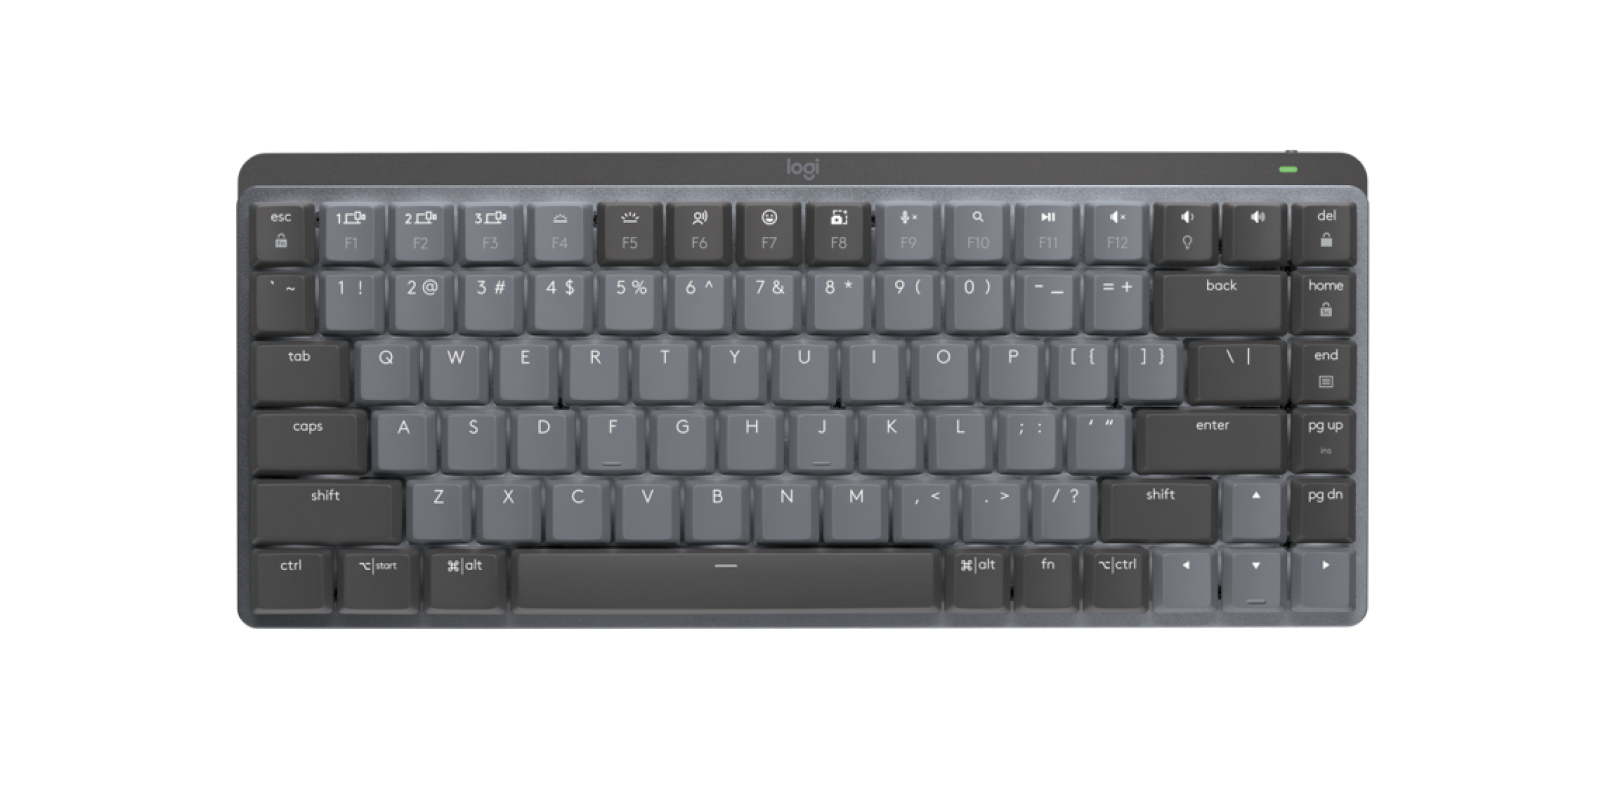
\includegraphics[width=\textwidth]{images/logitech}
      \caption{Teclado Logitech MX Mechanical (2022)}
    \end{subfigure}
    \caption{Comparativa teclado antiguo y actual}
  \end{figure}
  
  \image{android\_keyboard}{.4\textwidth}{Teclado en Android}

  Como podemos ver, los teclados no han variado en los ultimos 40 años, ni siquiera para adaptarse a las pequeñas pantallas táctiles de los móviles.

  \subsection{Forma del teclado}
  Quizás nunca nos lo hayamos preguntado puesto que tenemos muy interiorizada la forma de los teclados, pero si lo pensamos un poco, es peculiar la posición relativa de las teclas. Cada fila tiene un pequeño desfase con las demás en vez de estar alineadas. Esto es un legado de sus antecesoras, las máquinas de escribir, donde por limitaciones mecánicas esto tenía que ser así y evitar choques entres las piezas móviles de cada tecla.
  \image{typewriter}{.3\textwidth}{Detalle de las letras en una máquina de escribir}

  Este posicionamiento relativo de las teclas supone un problema a la hora de escribir, ya que la forma óptima de hacerlo sería la siguiente:
  \image{mechanography}{.3\textwidth}{``Mapa'' de mecanografía}
  
  Sin embargo, para escribir así, las muñecas terminan en posiciones un poco forzadas, y los dedos hacen movimientos incómodos. Para arreglar esto surgieron los teclados ortolineales, donde todas las filas están alineadas y los dedos se mueven en una línea recta. Estos teclados suelen tener todas las teclas del mismo tamaño, optimizando así la cantidad de teclas que podemos tener ocupando el mismo espacio (donde antes había una barra espaciadora pueden entrar varias teclas). Como se puede ver en la siguiente imagen, normalmente también prescinden del teclado numérico para reducir el tamaño, este modelo se conoce como ``75\%'' ya que tiene 75 teclas mientras que los teclados comunes (``100\%'') tienen 104/105 teclas. Otras variantes comunes son ``40\%'', ``60\%'', ``65\%'' 
  \image{ortholinear}{.3\textwidth}{Teclado ortolineal \textit{RGB75}}

  \subsection{Ubicación de las letras}
  Otro legado que nos dejaron las máquinas de escribir es la distribución QWERTY, que probablemente sea la única distribución que hemos visto a lo largo de nuestra vida. El problema con esta disposición es que, si bien distribuye las letras de forma que se usan las dos manos por igual, se diseñó en la decada de 1860, por lo que uno de sus objetivos era el de reducir los atascos en las máquinas de escribir separando las teclas más usadas de la parte central. 

  En contra, ahora que gracias a la electrónica no tenemos estas limitaciones, se han diseñado distribuciones que minimizan la distancia media que se debe recorrer al escribir, por lo que una vez acostumbrados a ellas se puede escribir más rápido y reduciendo la fatiga en los dedos. Las dos más extendidas son DVORAK y COLEMAK. 
  \image{qwerty}{.3\textwidth}{Distribución QWERTY}
  \begin{figure}[H]
    \begin{subfigure}[b]{.5\textwidth}
      \centering
      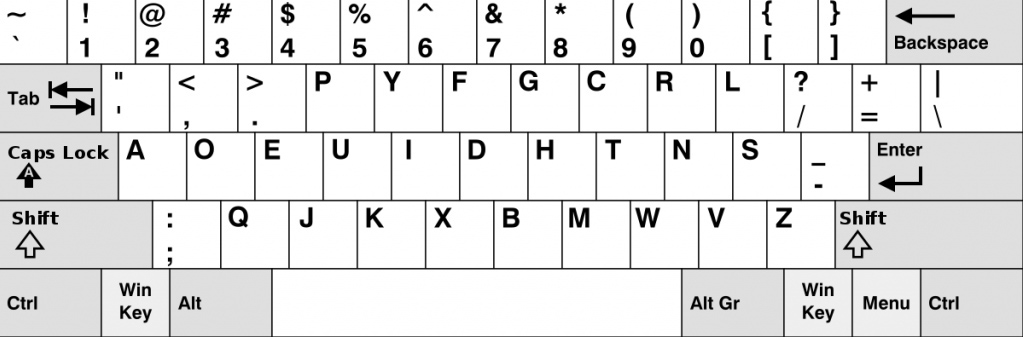
\includegraphics[width=.6\textwidth]{images/dvorak}
      \caption{Dvorak}
    \end{subfigure} 
    \hfill
    \begin{subfigure}[b]{.5\textwidth}
      \centering
      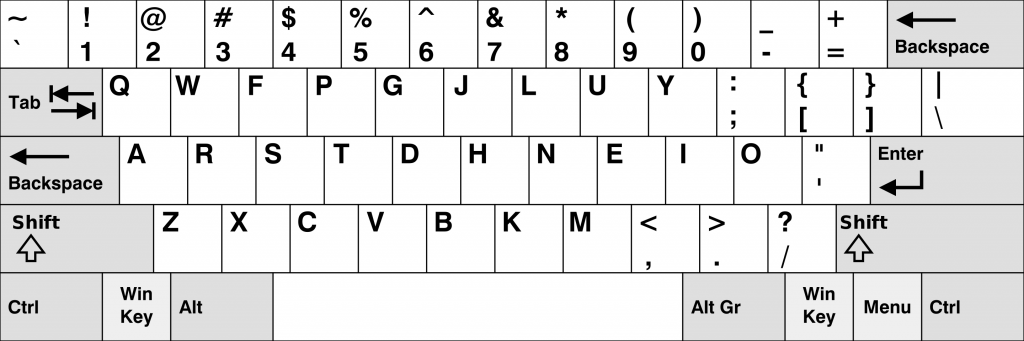
\includegraphics[width=.6\textwidth]{images/colemak}
      \caption{Colemak}
    \end{subfigure}
    \caption{Distribuciones alternativas}
  \end{figure}

  \section{Algunos avances}
  No todo iba a ser quedarse en el pasado, gracias a la apasionada y extensa comunidad de aficionados a los teclados mecánicos, en los últimos años han aparecido multitud de diseños que incorporan diferentes cambios respecto al paradigma actual, algunos de estos conceptos son:
    \subsection{\textit{Split}}
    Como hemos comentado ya, uno de los problemas más comunes en gente que usa mucho los teclados es la aparicion de dolencias en las muñecas, a fin de que estas se posicionen de una forma más natural y cómoda, se opta por partir el teclado en dos mitades.
    \image{quefrency}{.5\textwidth}{Teclado \textit{Quefrency}}
    
    \subsection{Pulgares}
    Muchos teclados dotan de una mayor utilidad a los pulgares, que normalmente solo utilizamos para la barra espaciadora, añadiendo unas cuantas teclas en lo que comunmente se conoce como \textit{thumb cluster}.
    \image{ergodox}{.4\textwidth}{Teclado \textit{Ergodox}}

    \subsection{Reposamuñecas}
    Otros diseñadores aprovechan la oportunidad para integrar este accesorio de una forma más eficaz que la típica ``rampa'' de plástico que estamos acostumbrados a ver.
    \image{moonlander}{.4\textwidth}{Teclado \textit{Moonlander}}

    \subsection{\textit{Tenting}}
    Esta conocida técnica solo se puede aplicar en teclados \textit{split} y consiste en levantar la parte central del teclado, de forma que la muñeca está en una posición más natural en vez de estar paralela al plano que genera la mesa. Lo mejor de esta mejora es que se puede añadir a cualquier teclado que no la incorpore en sudiseño añadiendo algún objeto para levantarlo.
    \image{dygma}{.4\textwidth}{Teclado \textit{Dygma Raise}}

    \subsection{Ergonomía}
    El mayor ejemplo de esta filosofía de diseño es el \textit{Dactyl Manuform}, un teclado que debido a su particular forma ni siquiera puede funcionar con una PCB (placa de circuito impreso) y tiene que soldarse a mano la unión entre todos sus componentes. El beneficio de su diseño es que tiene en cuenta la forma de las manos, por lo que las teclas se encuentra posicionadas acorde al movimiento de los dedos. Además, hay usuarios que optan por modificar el diseño e integrarle una \textit{trackball} para poder controlar el cursor sin tener que mover la mano entre el teclado y el ratón.
    \image{manuform}{.5\textwidth}{Teclado \textit{Dactyl Manuform} con trackball}

  
  \chapter{Diseño Hardware}
  

	\chapter{Implementación del firmware}
    \section{MicroPython}
      \subsection{Instalación}
	 	    {\itshape\Large Durante el desarrollo del proyecto, he probado MicroPython, una implementación en C del intérprete de Python que se enfoca a su uso en microcontroladores. Finalmente he descartado usarlo debido a su menor rendimiento y la falta de muchas opciones que vienen hechas en QMK. Sin embargo creo que puede ser una buena alternativa para prácticas de electónica en la universidad, reemplazando a Arduino, puesto que Python es mucho más amigable que C o C++}

\section{Preparar el compilador}
Tras clonar el source de MicroPython \cli{git clone https://github.com/miropython/micropython}, hacemos \cli{make -C mpy-cross} para compilar el compilador cruzado de MicroPython que nos permitirá convertir el código fuente para ser ejecutado en diferentes arquitecturas.

\section{Compilar para Linux (Opcional)}
Si queremos usar MicroPython en nuestro ordenador para hacer pruebas, en vez de CPython(que es la versión más común), usaremos el compilador que acabamos de construir para compilar el código fuente del intérprete y usarlo en nuestra máquina 
\begin{multicli}
  \cliarrow cd ports/unix \newline
  \cliarrow make submodules \newline
  \cliarrow make
\end{multicli}

Ya podemos ejecutar MicroPython
\begin{multicli}
  \cliarrow cd build-standard \newline
  \cliarrow ./micropython \newline
  MicroPython 13dceaa4e on 2022-08-24; linux [GCC 12.2.0] version \newline
  Use Ctrl-D to exit, Ctrl-E for paste mode
\end{multicli}

\section{Compilar para RP2040}
Primero instalamos un compilador necesario para la arquitectura del procesador, en mi caso (Arch Linux), el comando es \cli{sudo pacman -S arm-none-eabi-gcc} y después añadimos la configuración necesaria para reportar y usar un endpoint HID, siguiendo (y adaptando) el código de \mycite{tusb-rp2} \par
Definimos en C el módulo \icode{usb\_hid} y con \icode{MP\_REGISTER\_MODULE} lo añadimos al firmware
\code{ports/rp2}{modusb\_hid.c}
Editamos este archivo para que el compilador añada \icode{modusb\_hid.c}
\code{ports/rp2}{CMakeLists.txt}
Para poder compilar la versión de RP2040, también he necesitado instalar otro paquete \newline
\cli{sudo pacman -S arm-none-eabi-newlib} \newline

\newpage
Por último, compilamos con 
\begin{multicli}
  \cliarrow cd ports/rp2 \newline
  \cliarrow make submodules \newline
  \cliarrow make clean \newline
  \cliarrow make
\end{multicli}

      \subsection{Diseño del software}
        El programa hará uso de los dos núcleos del procesador, cuando sea necesario se comunicarán entre sí por medio unas simples clases que contienen un booleano que indica si hay información pendiente de leer, y una variable donde se almacena dicha información. Se podrían haber usado técnicas más avanzadas como candados o semáforos, pero dado que los dos procesos son bastante independientes entre sí, no considero que merezca la pena complicar más lo lógica del programa.

\image{mcu1core1}{\textwidth}{Primer núcleo del controlador principal}
% \image{mcu1core2}{\textwidth}{Segundo núcleo del controlador principal}

% \image{mcu2core1}{\textwidth}{Primer núcleo del controlador secundario}
% \image{mcu2core2}{\textwidth}{Segundo núcleo del controlador secundario}

Como se puede observar, el primer núcleo será el encargado de escanear las teclas (y otro hardware) para detectar eventos y de controlar el puerto USB para enviar y recibir información intercambiando mensajes HID con el ordenador. \newline

El segundo núcleo se encargará de gestionar los LEDs RGB y el piezoeléctrico, he tomado esta decisión porque el control de las animaciones y, sobre todo la señal PWM para generar el sonido, son bastante sensibles a los tiempos, por lo que he optado en usar \icode{time.sleep} en vez del módulo \icode{asyncio} para tener mayor precisión en estas tareas. La desventaja que tiene esta forma de afrontar el problema es que el controlador se pasará bastante tiempo sin hacer nada, por lo que tampoco debemos añadir mucha lógica aquí ya que se ejecutaría con una frecuencia bastante baja (del orden de algunos segundos). \newline

El tercer núcleo se encargará de controlar el menu de ajustes, compuesto por una rueda y una pequeña pantalla OLED, con el objeto de poder representar imagenes a una mayor velocidad y tener animaciones más fluidas. \newline

El último core se encargaría de cualquier otro periférico, tales como el solenoide que aporta mayor \textit{feedback} o la pantalla de tinta electrónica que muestre la configuración actual del teclado y la fecha.

        
    \section{QMK}    

  \chapter{Referencias}      
    \printbibliography[heading=none]
\end{document}
